% Created 2018-11-18 dom 17:30
% Intended LaTeX compiler: pdflatex
\documentclass[xcolor={usenames,svgnames,dvipsnames}]{beamer}
\usepackage[utf8]{inputenc}
\usepackage[T1]{fontenc}
\usepackage{graphicx}
\usepackage{grffile}
\usepackage{longtable}
\usepackage{wrapfig}
\usepackage{rotating}
\usepackage[normalem]{ulem}
\usepackage{amsmath}
\usepackage{textcomp}
\usepackage{amssymb}
\usepackage{capt-of}
\usepackage{hyperref}
\usepackage{color}
\usepackage{listings}
\usepackage{mathpazo}
\usepackage{gensymb}
\usepackage{amsmath}
\usepackage{chemarr}%flechas para reacciones químicas (SFER.tex)
\bibliographystyle{plain}
\AtBeginSubsection[]{\begin{frame}[plain]\tableofcontents[currentsubsection,sectionstyle=show/shaded,subsectionstyle=show/shaded/hide]\end{frame}}
\AtBeginSection[]{\begin{frame}[plain]\tableofcontents[currentsection,hideallsubsections]\end{frame}}
\usepackage[emulate=units]{siunitx}
\sisetup{fraction=nice, decimalsymbol=comma, retain-unity-mantissa = false}
\newunit{\wattpeak}{Wp}
\newunit{\watthour}{Wh}
\newunit{\amperehour}{Ah}
\usepackage{steinmetz}
\hypersetup{colorlinks=true, linkcolor=Blue, urlcolor=Blue}
\renewcommand{\thefootnote}{\fnsymbol{footnote}}
\beamertemplatenavigationsymbolsempty
\setbeamertemplate{footline}[frame number]
\setbeamercolor{alerted text}{fg=blue!50!black} \setbeamerfont{alerted text}{series=\bfseries}
\usetheme[hideothersubsections]{Goettingen}
\usecolortheme{rose}
\usefonttheme{serif}
\author{Oscar Perpiñán Lamigueiro}
\date{\url{http://oscarperpinan.github.io}}
\title{Radiación Solar}
\subtitle{Energía Solar Fotovoltaica}
\hypersetup{
 pdfauthor={Oscar Perpiñán Lamigueiro},
 pdftitle={Radiación Solar},
 pdfkeywords={},
 pdfsubject={},
 pdfcreator={Emacs 25.2.2 (Org mode 9.1.13)}, 
 pdflang={Spanish}}
\begin{document}

\maketitle

\section{Introducción}
\label{sec:orgf4b380f}

\begin{frame}[label={sec:orgf2ca954}]{Radiación Solar y Sistemas Fotovoltaicos}
\begin{itemize}
\item La \alert{energía producida} por un sistema fotovoltaico depende principalmente de la \alert{radiación incidente} en el generador.

\item Consecuentemente, la \alert{estimación del comportamiento} de un sistema FV en un determinado lugar durante un período temporal exige \alert{conocer la radiación solar disponible en el plano del generador}.
\end{itemize}

\begin{center}
\includegraphics[width=.9\linewidth]{../figs/GCPVScheme.pdf}
\end{center}
\end{frame}

\begin{frame}[label={sec:org5405a20}]{La radiación solar no se puede calcular analíticamente}
\begin{itemize}
\item La radiación solar que alcanza la superficie terrestre es el resultado de complejas interacciones en la atmósfera.
\item Para estimar la radiación se requiere medidas terrestres o imágenes de satélite.
\end{itemize}
\begin{center}
\includegraphics[height=0.5\textheight]{../figs/SolarRadiationComponents_NREL.png}
\end{center}
\end{frame}

\begin{frame}[label={sec:org2f104d1}]{Ángulo de Inclinación}
\begin{itemize}
\item Los generadores FV tienen un \alert{ángulo de inclinación positivo} para maximizar el rendimiento.
\item Este ángulo depende de la \alert{latitud} del lugar y de la \alert{aplicación del sistema}.
\end{itemize}

\begin{center}
\includegraphics[height=0.5\textheight]{../figs/PVUrban.png}
\end{center}
\end{frame}

\begin{frame}[label={sec:orgc085208}]{Bases de Datos de Radiación Solar}
\begin{itemize}
\item Por tanto, es inviable mantener una base de datos de radiación solar \alert{incidente}.
\item Las \alert{bases de datos} registran radiación en el \alert{plano horizontal}.
\item La estimación de la radiación incidente en el plano inclinado requiere un \alert{procedimiento de transposición}.
\end{itemize}
\end{frame}


\begin{frame}[label={sec:org01836b7}]{Del plano horizontal al plano inclinado}
\begin{center}
\includegraphics[width=.9\linewidth]{../figs/ProcedimientoCalculoRadiacionInclinada.pdf}
\end{center}
\end{frame}

\section{Geometría Sol y Tierra}
\label{sec:org5f40095}
\subsection{Movimiento Sol-Tierra}
\label{sec:org3f89562}

\begin{frame}[label={sec:org5169428}]{Movimiento terrestre}
\begin{center}
\includegraphics[width=.9\linewidth]{../figs/PlanoEcliptica.pdf}
\end{center}

\begin{itemize}[<+->]
\item La Tierra \alert{gira sobre si misma} alrededor de su eje polar.
\begin{itemize}[<.->]
\item Periodo aproximado: 24 horas.
\end{itemize}

\item La Tierra se mueve \alert{alrededor del Sol} siguiendo una elipse de baja
excentricidad.
\begin{itemize}[<.->]
\item Periodo aproximado: 1 año.

\item Este movimiento está contenido en el llamado \emph{plano de la
eclíptica}
\end{itemize}
\end{itemize}
\end{frame}

\begin{frame}[label={sec:orgd2ebe7f}]{Movimiento terrestre}
\begin{center}
\includegraphics[width=.9\linewidth]{../figs/PlanoEcliptica.pdf}
\end{center}

\begin{itemize}
\item Entre el eje polar y el plano de la eclíptica hay un ángulo constante de \(23,45\degree\).

\item Entre el plano ecuatorial y la linea que une la Tierra y el Sol hay un ángulo variable: \emph{declinación.}
\end{itemize}
\end{frame}



\subsection{Ángulos Solares}
\label{sec:org9c115bc}

\begin{frame}[plain,label={sec:org30c98da}]{Ejes terrestres}
\begin{columns}
\begin{column}{0.6\columnwidth}
\begin{center}
\includegraphics[width=.9\linewidth]{../figs/SoldesdeTierra.pdf}
\end{center}
\end{column}

\begin{column}{0.6\columnwidth}
\begin{center}
\includegraphics[width=.9\linewidth]{../figs/SistemaCoordenadasTerrestre-crop.pdf}
\end{center}
\end{column}
\end{columns}

\begin{itemize}
\item \alert{Declinación}, \(\delta\): ángulo entre el plano ecuatorial y la linea que une la Tierra y el Sol.
\item \alert{Hora Solar}, \(w\): diferencia entre instante en curso y el mediodía solar (\(w = 0\)).
\end{itemize}
\end{frame}

\begin{frame}[label={sec:org9e88886}]{Declinación}
\begin{center}
\includegraphics[height=0.6\textheight]{../figs/Declinacion.pdf}
\end{center}

\begin{block}{Ecuación de Cooper}
\[\delta=23,45\degree\cdot\sin\left(\frac{2\pi\cdot\left(d_{n}+284\right)}{365}\right)\]
\end{block}
\end{frame}


\begin{frame}[label={sec:org85308e8}]{Estaciones}
\begin{itemize}[<+->]
\item \alert{Solsticio de junio} 
\begin{itemize}[<.->]
\item 21-22 Junio, \(d_n = 172-173\)

\item Declinación máxima.

\item Días más largos en hemisferio Norte (verano)

\item El Sol amanece por el Noreste y anochece por el Noroeste en el
hemisferio Norte.
\end{itemize}

\item \alert{Solsticio de diciembre} 
\begin{itemize}[<.->]
\item 21-22 Diciembre, \(d_n = 355-356\)

\item Declinación mínima.

\item Días más cortos en hemisferio Norte (invierno)

\item El Sol amanece por el Sureste y anochece por el Suroeste en el
hemisferio Norte.
\end{itemize}

\item \alert{Equinoccios} 
\begin{itemize}[<.->]
\item 21-22 Marzo (\(d_n = 80-81\))

\item 22-23 Septiembre (\(d_n = 265-266\))

\item Declinación nula

\item La duración de noche y día coinciden.

\item El Sol amanece por el Este y anochece por el Oeste.
\end{itemize}
\end{itemize}
\end{frame}

\begin{frame}[label={sec:org12bd358}]{Hora Solar}
\begin{itemize}
\item \(w\), diferencia entre instante en curso y el mediodía solar (\(w = 0\), \(\psi_s = 0\)).
\item Criterio de signos: \(w < 0\) antes del mediodía.
\item 1h = 15º (\(24\text{h} = 2\pi \text{ radians} = 360\))
\item (Horas) \(-12, -11, -10, \dots, -1, \textbf{0}, 1, \dots, 10, 11, 12\)
\end{itemize}

\begin{block}{Amanecer (\(\gamma_{s}=0\))}
\[
\cos(\omega_{s}) = -\tan(\delta)\tan(\phi)
\]

La longitud del día, \(|2 \cdot \omega_s|\), depende de \(\phi\) y \(d_n\).
\end{block}
\end{frame}

\begin{frame}[label={sec:org191e29a}]{Duración del día}
\begin{center}
\includegraphics[width=.9\linewidth]{../figs/DuracionDia.pdf}
\end{center}
\end{frame}

\begin{frame}[plain,label={sec:orgbc37073}]{Ejes locales}
\begin{columns}
\begin{column}{0.6\columnwidth}
\begin{center}
\includegraphics[width=.9\linewidth]{../figs/SoldesdeTierra2.pdf}
\end{center}
\end{column}

\begin{column}{0.6\columnwidth}
\begin{center}
\includegraphics[width=.9\linewidth]{../figs/SistemaCoordenadasLocal-crop.pdf}
\end{center}
\end{column}
\end{columns}

\begin{itemize}
\item \alert{Cenit Solar}, \(\theta_{zs}\): ángulo entre el Sol y el cenit (vertical en un lugar determinado).
\item \alert{Azimut Solar}, \(\psi_s\): ángulo entre el mediodía solar y la proyección del sol en el plano horizontal.
\item Dependen de \(d_n\), \(\omega\), y \(\phi\).
\end{itemize}
\end{frame}


\begin{frame}[label={sec:orgc734592}]{Relación entre sistemas de coordenadas}
\begin{center}
\includegraphics[width=.9\linewidth]{../figs/RelacionSistemasCoordenadas.pdf}
\end{center}

\begin{itemize}
\item \alert{Latitud (\(\phi\)) con signo}: Positivo para Hemisferio Norte, Negativo para Hemisferio Sur.
\end{itemize}
\end{frame}

\begin{frame}[plain,label={sec:org54352f8}]{Cenit Solar}
\[
\cos(\theta_{zs}) = \cos(\delta) \cos(\omega) \cos(\phi) + \sin(\delta) \sin(\phi)
\]

\begin{columns}
\begin{column}{0.55\columnwidth}
\begin{itemize}
\item \(\theta_{zs}\), ángulo entre el Sol y el cenit (vertical en un lugar determinado).
\item \(\gamma_s\), altura solar, ángulo complementario de \(\theta_{zs}\).
\item Depende de \(d_n\), \(\omega\), y \(\phi\).
\end{itemize}
\end{column}
\begin{column}{0.75\columnwidth}
\begin{center}
\includegraphics[width=.9\linewidth]{../figs/SistemaCoordenadasLocal-crop.pdf}
\end{center}
\end{column}
\end{columns}
\end{frame}

\begin{frame}[plain,label={sec:org3f771e3}]{Azimut solar}
\[
  \cos(\psi_{s}) = \mathrm{sign}(\phi) \cdot \frac{\cos(\delta) \cos(\omega) \sin(\phi) - \cos(\phi) \sin(\delta)} {\sin(\theta_{z})}
\]
\begin{columns}
\begin{column}{0.55\columnwidth}
\begin{itemize}
\item \(\psi_s\), ángulo entre el mediodía solar y la proyección del sol en el plano horizontal.
\item Depende de \(d_n\), \(\omega\), y \(\phi\).
\item Criterio de Signos: negativo antes del mediodía.
\end{itemize}
\end{column}

\begin{column}{0.7\columnwidth}
\begin{center}
\includegraphics[width=.9\linewidth]{../figs/SistemaCoordenadasLocal-crop.pdf}
\end{center}
\end{column}
\end{columns}
\end{frame}

\begin{frame}[label={sec:org4346218}]{Trayectoria Solar (\(60\degree N\))}
\begin{center}
\includegraphics[width=.9\linewidth]{../figs/TrayectoriaSolar60N.pdf}
\end{center}
\end{frame}


\begin{frame}[label={sec:org84ff270}]{Trayectoria Solar (\(40\degree S\))}
\begin{center}
\includegraphics[width=.9\linewidth]{../figs/TrayectoriaSolar40S.pdf}
\end{center}
\end{frame}


\begin{frame}[label={sec:orgdea330e}]{Cálculo Ángulos Solares}
\begin{itemize}
\item Azimut, Ángulo Cenital y Altura Solar, Duración del Dia para el:

\begin{itemize}
\item Día del Año: 120, 2 horas después del mediodía, Latitud: 37.2N

\item Día del Año: 340, 2 horas después del amanecer, Latitud: 15S
\end{itemize}

\item Duración del día 261 del año en las latitudes 10N, 40N, 70N, 10S,
40S, 70S.

\item Altura solar en el mediodía del día 25 del año en las latitudes 10N,
40N, 10S, 40S.
\end{itemize}
\end{frame}

\subsection{Hora solar y oficial}
\label{sec:orgbca83d9}
\begin{frame}[label={sec:org983cd08}]{Hora solar}
\[\omega=15\cdot(\mathrm{TO}-\mathrm{AO}-12)+\Delta\lambda+\frac{\mathrm{EoT}}{4}\]

\begin{itemize}
\item \(\omega\): hora solar real o aparente[º]
\item \(TO\): hora oficial [h]
\item \(AO\): adelanto oficial por horario de verano [h]
\item \(\Delta\lambda\) corrección por huso horario [º]
\item \(EoT\): Ecuación del tiempo (dia solar real y dia solar medio) [min]
\end{itemize}
\end{frame}

\begin{frame}[label={sec:orga9f8092}]{Hora oficial}
\begin{itemize}
\item \alert{La hora oficial} es una medida del tiempo \alert{ligada a un meridiano}
que sirve de referencia para una zona determinada.

\item La hora oficial de la España peninsular se rige por el huso horario
de Centroeuropa. Este huso horario está situado en
\(15\degree\mathrm{E}\).

\item \alert{Corrección}: \(\Delta\lambda=\lambda_{L}-\lambda_{H}\), con
\(\lambda_{L}\) la longitud local y \(\lambda_{H}\) la longitud del huso
horario.

\item Longitudes \emph{positivas} al \emph{este} del meridiano de Greenwich.
\(\Delta\lambda\) es positiva cuando la localidad está situada al este
de su huso horario.
\end{itemize}
\end{frame}

\begin{frame}[label={sec:orgfa6d5c7}]{Tiempo solar medio}
\begin{itemize}
\item \alert{La duración del día solar real}, definido como el tiempo que
transcurre entre dos pasos consecutivos del Sol por el meridiano
local, \alert{varía a lo largo del año}.

\item El promedio anual de esta variación es nulo: \emph{día solar medio}, cuya
duración es constante a lo largo del año e igual al valor medio de la
duración del día solar real.
\end{itemize}
\end{frame}

\begin{frame}[label={sec:org3c727d0}]{Ecuación del Tiempo}
\[
\mathrm{EoT}=229.18\cdot\left(-0.0334\cdot\sin(M)+0.04184\cdot\sin\left(2\cdot
      M+3.5884\right)\right)
\]
\[
M=\frac{2\pi}{365.24}\cdot d_{n}
\]
\begin{center}
\includegraphics[width=.9\linewidth]{../figs/EoT.pdf}
\end{center}
\end{frame}

\begin{frame}[label={sec:orga5d79cc}]{Ejemplo de cálculo}
\[\omega=15\cdot(\mathrm{TO}-\mathrm{AO}-12)+\Delta\lambda+\frac{\mathrm{EoT}}{4}\]

\begin{block}{}
Calcule la hora solar real correspondiente al día 23 de Abril de 2010
  (\(\mathrm{EoT=\SI{1.78}{\minute}}\)) a las 12 de la mañana, hora
  oficial de la ciudad de A Coruña, Galicia. Esta localidad está
  contenida en el meridiano de longitud \(8.38\degree\mathrm{W}\) y su
  hora oficial está regida por el huso horario GMT+1.
\end{block}
\end{frame}

\begin{frame}[label={sec:org1a676c8}]{Solución}
\[\omega=15\cdot(\mathrm{TO}-\mathrm{AO}-12)+\Delta\lambda+\frac{\mathrm{EoT}}{4}\]

\begin{itemize}[<+->]
\item \(\lambda_{L}=-8.38\degree\), \(\lambda_{H}=15\degree\) y
\(\Delta\lambda=-23.38\degree\).

\item En España se aplica el horario de verano y este día está incluido
en el período afectado, \(\mathrm{AO}=1\).

\item Por último, para este día \(\mathrm{EoT=\SI{1.78}{\minute}}\).

\item Así \(\omega=-37.94\degree\) (aproximadamente las 9 y media de la
mañana). El Sol culminará (\(\omega=0\)) cuando sean las 14:31, hora
oficial.
\end{itemize}
\end{frame}

\section{Geometría de los sistemas fotovoltaicos}
\label{sec:org4bdc34f}
\begin{frame}[label={sec:orgadd017e}]{Definiciones}
\begin{itemize}
\item \(\theta_s\), ángulo de incidencia (AOI), ángulo entre los rayos solares y la perpendicular al plano del generador.
\item \(\alpha\): orientación del generador (0º cuando está orientado al mediodía solar)
\item \(\beta\): inclinación del generador (respecto de la superficie horizontal)
\end{itemize}
\end{frame}

\subsection{Sistema Estático}
\label{sec:org0bbe959}

\begin{frame}[label={sec:org0b81b8d}]{Sistema Estático}
\begin{center}
\includegraphics[width=.9\linewidth]{../figs/EstructuraEstaticaSuelo.jpg}
\end{center}
\end{frame}

\begin{frame}[plain,label={sec:org272b0b0}]{Ángulo de Incidencia}
\begin{itemize}
\item Si \(\alpha=0\)
\end{itemize}
\[
\cos(\theta_{s}) = \cos(\delta)\cos(\omega)\cos(\beta-|\phi|)- \mathrm{sign}(\phi)\cdot\sin(\delta)\sin(\beta-|\phi|)
\]

\begin{center}
\includegraphics[height=0.6\textheight]{../figs/AngulosSistemaEstatico.pdf}
\end{center}

\begin{itemize}
\item Inclinación Óptima \(\beta_{opt} \simeq |\phi| - 10º\).
\end{itemize}
\end{frame}

\begin{frame}[label={sec:org747fe0a}]{Ángulo de Incidencia}
\begin{itemize}
\item \(40\degree N\)
\end{itemize}
\begin{center}
\includegraphics[height=0.8\textheight]{../figs/cosThetaEst_40N.pdf}
\end{center}
\end{frame}


\subsection{Sistemas con seguimiento}
\label{sec:org76d0b0b}

\begin{frame}[label={sec:orgee12233}]{Introducción}
\begin{itemize}[<+->]
\item \alert{Fundamento:}
\begin{itemize}[<.->]
\item Radiación incidente aumenta al seguir al sol

\item Pérdidas por reflexión disminuyen si el apuntamiento al sol mejora
\end{itemize}

\item Las diferentes técnicas de seguimiento son un \alert{compromiso} entre
\begin{itemize}[<.->]
\item un \alert{apuntamiento perfecto}

\item \alert{sistemas estructurales más económicos}

\item mejores \alert{aprovechamientos del terreno}.
\end{itemize}
\end{itemize}
\end{frame}
\begin{frame}[label={sec:orga7ad622}]{Algunos tipos de seguimiento solar}
\begin{itemize}[<+->]
\item \alert{Doble eje}
\begin{itemize}[<.->]
\item Apuntamiento \guillemotleft{}perfecto\guillemotright{}

\item Mejor productividad, peor ocupación de terreno.
\end{itemize}

\item \alert{Seguimento acimutal}
\begin{itemize}[<.->]
\item Sacrifica un movimiento (inclinación del generador) para conseguir
sistemas más económicos.
\end{itemize}

\item \alert{Seguimiento horizontal con eje Norte-Sur}
\begin{itemize}[<.->]
\item Sencillez y estabilidad estructural (el eje es horizontal y
paralelo al terreno, con tantos puntos de apoyo como se consideren
necesarios),

\item Facilidad de motorización,

\item Buen aprovechamiento del terreno.
\end{itemize}
\end{itemize}
\end{frame}

\begin{frame}[label={sec:org9f9eb5e}]{Sistema de Seguimiento(1 eje, horizontal N-S)}
\begin{center}
\includegraphics[width=.9\linewidth]{../figs/SeguidorEjeHorizontal.jpg}
\end{center}
\end{frame}


\begin{frame}[plain,label={sec:org2cd6ec0}]{Ángulo de Incidencia (1x eje, horizontal N-S)}
\[\cos(\theta_{s})=\cos(\delta)\sqrt{\sin^{2}(\omega)+\left(\cos(\omega)\cos(\phi)+\tan(\delta)\sin(\phi)\right)^{2}}\]

\begin{center}
\includegraphics[height=0.6\textheight]{../figs/AngulosSistemaHorizontalNS.pdf}
\end{center}
\end{frame}

\begin{frame}[label={sec:orgae3cd51}]{Inclinación de Eje Horizontal N-S}
\begin{itemize}
\item \(40\degree N\)
\end{itemize}
\begin{center}
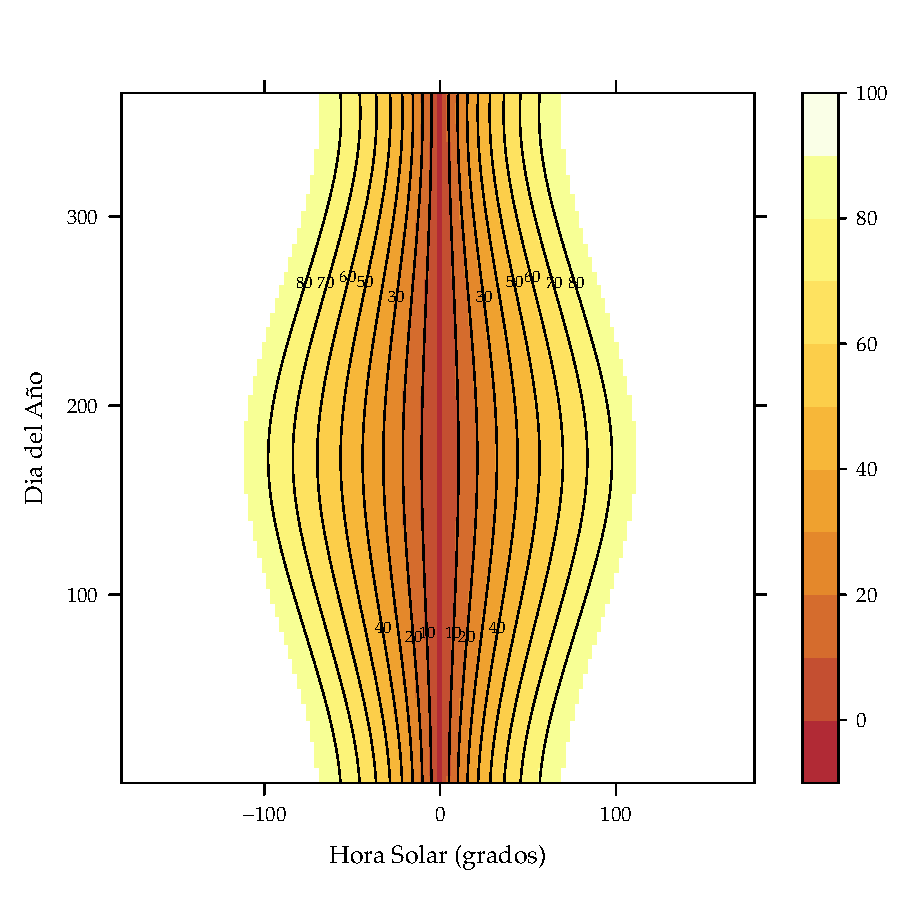
\includegraphics[height=0.8\textheight]{../figs/BetaHoriz_40N.pdf}
\end{center}
\end{frame}



\begin{frame}[label={sec:org3b3e1ed}]{Ángulo de Incidencia de Eje Horizontal N-S}
\begin{itemize}
\item \(40\degree N\)
\end{itemize}
\begin{center}
\includegraphics[height=0.8\textheight]{../figs/cosThetaHoriz_40N.pdf}
\end{center}
\end{frame}




\begin{frame}[label={sec:org0a10378}]{Sistema de Seguimiento (2x ejes)}
\begin{center}
\includegraphics[width=.9\linewidth]{../figs/SeguidorReocin.jpg}
\end{center}
\end{frame}

\begin{frame}[plain,label={sec:org32114ca}]{Ángulo de Incidencia (seguidor 2x)}
\begin{center}
\includegraphics[width=.9\linewidth]{../figs/Sombra2X.pdf}
\end{center}


\begin{align*}
  \beta &= \theta_{z}\\
  \alpha &= \psi_{s}\\
  \cos(\theta_{s}) &= 1
\end{align*}
\end{frame}
\begin{frame}[label={sec:org61a811e}]{Inclinación (seguidor 2x)}
\begin{itemize}
\item \(40\degree N\)
\end{itemize}
\begin{center}
\includegraphics[height=0.8\textheight]{../figs/BetaDoble_40N.pdf}
\end{center}
\end{frame}

\begin{frame}[label={sec:orgf57cfb6}]{Ejercicio: cálculo de ángulo de incidencia}
\begin{description}
\item[{Para:}] \begin{itemize}
\item Un sistema estático orientado al Sur y con inclinación de 30;

\item Un sistema de seguimiento horizontal N-S;

\item Un sistema de seguimiento acimutal con inclinación a 35;

\item Un sistema de seguimiento a doble eje,
\end{itemize}

\item[{Calcular}] el ángulo de incidencia para el:

\begin{itemize}
\item Día del Año: 120, 2 horas después del mediodía, Latitud: 37.2N;

\item Día del Año: 340, 2 horas después del amanecer, Latitud: 15S;
\end{itemize}
\end{description}
\end{frame}
\section{Radiación Solar en la Superficie Terrestre}
\label{sec:org92d06d5}
\begin{frame}[label={sec:orgbd69fae}]{Irradiancia e Irradiación}
\begin{description}
\item[{Irradiancia}] es la densidad de \emph{potencia} de radiacion solar
incidente en una superficie.

\begin{itemize}
\item Unidades: \(\si{\watt\per\meter\squared},\,\si{\kilo\watt\per\meter\squared}\)
\end{itemize}

\item[{Irradiación}] es la densidad de \emph{energía} de radiación solar
incidente en una superficie.

\begin{itemize}
\item Unidades: \(\si{\watthour\per\meter\squared},\,\si{\kilo\watthour\per\meter\squared}\)
\end{itemize}
\end{description}
\end{frame}

\subsection{Radiación Extra-atmosférica}
\label{sec:org45b060d}


\begin{frame}[label={sec:org1feebc2}]{Definición}
\begin{itemize}
\item La radiación que alcanza la superficie de la atmósfera es radiación
directa del Sol.
\end{itemize}

\begin{center}
\includegraphics[height=0.5\textheight]{../figs/SolarRadiationComponents_NREL.png}
\end{center}
\end{frame}


\begin{frame}[label={sec:orgd6cc47c}]{Ecuaciones}
\begin{itemize}
\item \alert{Constante solar} \(B_{0}=\SI{1367}{\watt\per\meter\squared}\)
(irradiancia solar sobre la superficie normal al vector solar en límite superior de la atmósfera terrestre)

\item \alert{Irradiancia extra-atmosférica}

\[B_{0}(0)=B_{0}\cdot\epsilon_{0}\cdot\cos\theta_{zs}\]

\item \alert{Irradiación extra-atmosférica diaria}  (\(\omega_{s}\) en radianes)
\[
  B_{0d}(0)=-\frac{24}{\pi}B_{0}\epsilon_{0}\cdot\left(\omega_{s}\sin\phi\sin\delta+\cos\delta\cos\phi\sin\omega_{s}\right)
\]

\item Factor de corrección por excentricidad
\[\epsilon_0 = 1+0,033\cdot\cos(2\pi d_n/365)\]
\end{itemize}
\end{frame}


\begin{frame}[label={sec:org304e9b6}]{Días promedio}
\begin{itemize}
\item Es posible demostrar que el \alert{promedio mensual} de esta irradiación
diaria \alert{coincide numericamente} con el valor de irradiación diaria
correspondiente a los denominados \alert{días promedios}, días en los que
la declinación correspondiente coincide con el promedio mensual

\item Por tanto, podemos calcular el valor medio mensual de la irradiación
diaria extra-atmosférica con el valor de la declinación de uno de los
doce días promedio.
\end{itemize}

\begin{center}
\begin{tabular}{lrrrrrr}
Mes & Ene & Feb & Mar & Abr & May & Jun\\
\hline
\(d_n\) & 17 & 45 & 74 & 105 & 135 & 161\\
\end{tabular}
\end{center}

\begin{center}
\begin{tabular}{lrrrrrr}
Mes & Jul & Ago & Sep & Oct & Nov & Dic\\
\hline
\(d_n\) & 199 & 230 & 261 & 292 & 322 & 347\\
\end{tabular}
\end{center}
\end{frame}

\subsection{Radiación solar en la superficie terrestre}
\label{sec:org7b96534}

\begin{frame}[label={sec:org17495b2}]{Interacción de la radiación con la atmósfera}
\begin{itemize}
\item \alert{Disminución} de la radiación incidente en la superficie terrestre
(reflexión en nubes)

\item \alert{Modificación de las características espectrales} de la radiación
(absorción por vapor de agua, ozono y CO2)

\item \alert{Modificación de la distribución espacial} (dispersión por
partículas)
\end{itemize}
\end{frame}

\begin{frame}[label={sec:org1b88f72}]{Caracterización de la atmósfera}
\begin{itemize}
\item \alert{Masa de aire}:

\begin{itemize}
\item Relación entre camino recorrido por rayos directos del Sol a
través de la atmósfera hasta la superficie receptora y el que recorrerían en caso de incidencia vertical (AM=1)

\item \(AM \simeq 1/\cos\theta_{zs}\)
\end{itemize}

\item \alert{Índice de claridad}

\begin{itemize}
\item Relación entre la radiación en la superficie terrestre y la
radiación extra-atmosférica, ambas en el plano horizontal

\item El índice de claridad \alert{no depende de las variaciones debidas al
movimiento aparente del sol}.

\item \(K_{Tm}=\frac{G_{d,m}(0)}{B_{0d,m}(0)}\) (mensual)
\end{itemize}
\end{itemize}
\end{frame}

\begin{frame}[label={sec:org8345c68}]{Índice de claridad}
\begin{description}
\item[{\(K_{T}\):}] índice de claridad instantáneo. \(K_{T}=G/B_{0}\)

\item[{\(K_{Td}\):}] índice de claridad diario. \(K_{Td}=G_{d}/B_{0d}\)

\item[{\(K_{Tm}\):}] índice de claridad mensual. \(K_{Tm}=G_{m}/B_{0m}=G_{d,m}/B_{0d,m}\)

\item[{\(K_{Ta}\):}] índice de claridad anual. \(K_{Ta} = G_{a}/B_{0a} = \dots\)
\end{description}
\end{frame}

\begin{frame}[label={sec:orgb48f574}]{Componentes de la radiación solar}
\begin{itemize}
\item \alert{Radiación Directa}. (B)

\begin{itemize}
\item Linea recta con el Sol.
\end{itemize}

\item \alert{Radiación Difusa}. (D)

\begin{itemize}
\item Procedente de todo el cielo salvo el Sol

\item Rayos dispersados por la atmósfera.

\item Anisotrópica, proceso estocástico.
\end{itemize}

\item \alert{Radiación del albedo}. (R, AL)

\begin{itemize}
\item Procedente del suelo (reflejada)
\end{itemize}

\item \alert{Radiación Global:} \(G=B+D+R\)
\end{itemize}
\end{frame}

\begin{frame}[label={sec:org0231ca1}]{Cómo se escribe}
\begin{block}{Forma, tiempo, lugar}
\begin{description}
\item[{Forma+Tiempo+Lugar:}] Irradiancia directa (forma) horaria (tiempo)
en el plano del generador (lugar)

\item[{Promedios:}] Media mensual (periodo) de la irradiación global
(forma) diaria (tiempo)

\item[{Lugar:}] (Orientación, Inclinación)

(0=Horizontal)

(n=Normal)

(I=Plano del generador)
\end{description}
\end{block}
\end{frame}

\begin{frame}[label={sec:org1aeec4c}]{Cómo se escribe}
\begin{block}{Forma, tiempo, lugar}
\[Forma_{tiempo,promedio}(lugar)\]

\[G_{d,m}(0)\]

\[D_{h}(\alpha,\beta)\]

\[B_{0d}(n)\]

\[B(\beta)\]
\end{block}
\end{frame}
\subsection{Cálculo de componentes de radiación solar}
\label{sec:org66d2ff3}

\begin{frame}[label={sec:org026a32d}]{}
\begin{center}
\includegraphics[width=.9\linewidth]{../figs/ProcedimientoCalculoRadiacionInclinada_componentes.pdf}
\end{center}
\end{frame}

\begin{frame}[label={sec:org96f36b5}]{Estimación de Directa y Difusa}
\begin{itemize}
\item Objetivo: Establecer una \alert{relación entre la fracción difusa} de la radiación horizontal (\(F_{D}=\frac{D(0)}{G(0)}\)) y \alert{el índice de claridad}.

\item \alert{Correlación negativa} (a mayor índice de claridad, menor componente difusa)

\item \alert{Correlación independiente de la latitud} (validez cuasi-universal)
\end{itemize}
\end{frame}

\begin{frame}[label={sec:orgbcefb27}]{Correlaciones \(F_{D}\) y \(K_{T}\): Ecuación de Page}
\begin{center}
\includegraphics[width=.9\linewidth]{../figs/FdKtMensual.pdf}
\end{center}

\[F_{Dm}=1-1.13\cdot K_{Tm}\]
\end{frame}

\begin{frame}[label={sec:org52c8d85}]{Correlaciones \(F_{D}\) y \(K_{T}\)}
Ejemplo: en un lugar con \(G_{d,m}(0) = \SI{3150}{\watthour\per\meter\squared}\) en un mes con \(B_{o,dm}(0) = \SI{4320}{\watthour\per\meter\squared}\)  será:

\begin{itemize}
\item \(K_{Tm}=\frac{3150}{4320}=0.73\)

\item Según la correlación de Page, \(F_{Dm}=1-1.13\cdot0.73=0.175\)

\item \(D_{d,m}(0)=0.175\cdot3150=\SI{551.6}{\watthour\per\meter\squared}\)

\item \(B_{d,m}(0)=3150-551.6=\SI{2598,4}{\watthour\per\meter\squared}\)
\end{itemize}
\end{frame}

\begin{frame}[label={sec:org4656096}]{Correlaciones \(F_{D}\) y \(K_{T}\): Collares-Pereira y Rabl}
\begin{center}
\includegraphics[width=.9\linewidth]{../figs/FdKtDiario.pdf}
\end{center}
{\scriptsize \[
F_{Dd} = \begin{cases}
  0.99 & K_{Td} \leq 0.17\\
  1.188 - 2.272 \cdot K_{Td} + 9.473 \cdot K_{Td}^{2} - 21.856 \cdot K_{Td}^{3} + 14.648 \cdot K_{Td}^{4} & K_{Td} > 0.17
\end{cases}
\]
}
{\scriptsize \par}
\end{frame}

\begin{frame}[label={sec:org514be12}]{Ejemplo}
\begin{description}
\item[{Calcular}] las componentes directa y difusa de la radiación solar del:

\begin{itemize}
\item Mes de Septiembre (día 261) en un lugar con latitud \(\phi=\ang{40}\mathrm{N}\) y con media mensual de irradiación global diaria horizontal
\(G_{d,m}(0)=\SI{2700}{\watthour\per\meter\squared}\).
\end{itemize}
\end{description}
\end{frame}
\section{Radiación Solar en Generadores FV}
\label{sec:org596a568}

\subsection{Introducción}
\label{sec:org93b0dda}

\begin{frame}[label={sec:orgf067128}]{Ángulo de Inclinación}
\begin{itemize}
\item Los generadores FV tienen un ángulo de inclinación positivo para maximizar el rendimiento.
\item Este ángulo depende de la latitud del lugar y de la aplicación del sistema.
\end{itemize}

\begin{center}
\includegraphics[height=0.5\textheight]{../figs/PVUrban.png}
\end{center}
\end{frame}

\begin{frame}[label={sec:org0d2d0bd}]{}
\begin{center}
\includegraphics[width=.9\linewidth]{../figs/ProcedimientoCalculoRadiacionInclinada_perfil.pdf}
\end{center}
\end{frame}

\subsection{Irradiancia a partir de irradiación diaria}
\label{sec:orge82f238}

\begin{frame}[label={sec:org4f3937f}]{Planteamiento}
\begin{itemize}
\item \alert{Objetivo}: construir un perfil diario promedio de irradiancia global e irradiancia difusa (\emph{cielo claro})
\item \alert{Puntos clave}:
\begin{itemize}
\item La variación solar durante una hora es baja: irradiación horaria equivale al valor medio de la irradiancia durante esa hora.
\item Relación entre irradiancia e irradiación extra-terrestre deducible teóricamente:
\end{itemize}
\end{itemize}

\[
\frac{B_{o}(0)}{B_{0d}(0)}=\frac{\pi}{24}\cdot\frac{\cos(\omega)-\cos(\omega_{s})}{\omega_{s}\cdot\cos(\omega_{s})-\sin(\omega_{s})}
\]
\end{frame}

\begin{frame}[label={sec:org165fb82}]{Perfil}
\begin{center}
\includegraphics[width=.9\linewidth]{../figs/RgRd.pdf}
\end{center}
\end{frame}

\begin{frame}[label={sec:orgccd20a9}]{Ecuaciones del perfil}
\[r_{D}=\frac{D(0)}{D_{d}(0)}=\frac{B_{o}(0)}{B_{0d}(0)}\]

\[r_{G}=\frac{G(0)}{G_{d}(0)}=r_{D}\cdot\left(a+b\cdot\cos(\omega)\right)\]

\[a=0.409-0.5016\cdot\sin(\omega_{s}+\frac{\pi}{3})\]

\[b=0.6609+0.4767\cdot\sin(\omega_{s}+\frac{\pi}{3})\]
\end{frame}

\begin{frame}[label={sec:org2918de6}]{Ejercicio}
\begin{description}
\item[{Calcular}] la irradiancia global y la irradiancia difusa en el plano horizontal

\begin{itemize}
\item 2 horas antes del mediodía del día 261 en un lugar con latitud \(\phi=\ang{40}\mathrm{N}\) y con media mensual de irradiación global diaria horizontal \(G_{d,m}(0)=\SI{2700}{\watthour\per\meter\squared}\).
\end{itemize}
\end{description}
\end{frame}

\subsection{Transformación al plano del generador}
\label{sec:orga25a0ae}

\begin{frame}[label={sec:orgeddb0ee}]{}
\begin{center}
\includegraphics[width=.9\linewidth]{../figs/ProcedimientoCalculoRadiacionInclinada_inclinada.pdf}
\end{center}
\end{frame}

\begin{frame}[label={sec:orgf2acab5}]{Planteamiento}
\begin{itemize}
\item \alert{Irradiancia Directa}: ecuación analítica basada en geometría solar (ángulo cenital) y del generador (ángulo de incidencia).
\item \alert{Irradiancia Difusa}: modelos del estado de cielo, modelo isotrópico o anisotrópico.
\item \alert{Irradiancia de Albedo}: modelo isotrópico con coeficiente de reflexión típico.
\end{itemize}
\end{frame}
\begin{frame}[label={sec:orgcc81ea2}]{Irradiancia Directa}
\alert{Irradiancia Directa}: ecuación analítica basada en geometría solar (ángulo cenital) y del generador (ángulo de incidencia).

\[B(\beta,\alpha)=B(0)\cdot\frac{\max(0,\cos(\theta_{s}))}{\cos(\theta_{zs})}\]
\end{frame}

\begin{frame}[label={sec:org51cf50f}]{Irradiancia Difusa}
\begin{center}
\includegraphics[width=.9\linewidth]{../figs/AnguloVisionCielo.pdf}
\end{center}

\[D(\beta,\alpha)=\intop_{\Omega}L(\theta_{z},\psi)\cdot\cos(\theta_{z}^{'})d\Omega\]
\end{frame}

\begin{frame}[label={sec:orgb346ba4}]{Irradiancia Difusa Isotrópica}
\begin{center}
\includegraphics[width=.9\linewidth]{../figs/AnguloVisionCielo.pdf}
\end{center}


\[L(\theta_{z},\psi)=cte.\]

\[D(\beta,\alpha)=D(0)\cdot\frac{1+\cos(\beta)}{2}\]
\end{frame}
\begin{frame}[label={sec:orgbca189e}]{Irradiancia Difusa Anisotrópica}
\[D(\beta,\alpha) = D^{I}(\beta,\alpha)+D^{C}(\beta,\alpha)\]

\[D^{I}(\beta,\alpha) = D(0) \cdot (1-k_{1}) \cdot \frac{1 + \cos(\beta)}{2}\]

\[D^{C}(\beta,\alpha) = D(0) \cdot k_{1} \cdot \frac{\max(0,\cos(\theta_{s}))}{\cos(\theta_{zs})}\]

\[k_{1} = \frac{B(0)}{B_{0}(0)}\]
\end{frame}

\begin{frame}[label={sec:org0288a6c}]{Irradiancia de Albedo}
\begin{center}
\includegraphics[width=.9\linewidth]{../figs/AnguloVisionCielo.pdf}
\end{center}


\[R(\beta,\alpha)=\rho\cdot G(0)\cdot\frac{1-\cos(\beta)}{2}\]

\[\rho=0.2\]
\end{frame}

\begin{frame}[label={sec:org089f84e}]{Ejercicio}
\begin{description}
\item[{Calcular}] la irradiancia difusa, directa, de albedo y global, en

\begin{itemize}
\item Un generador inclinado \(\ang{30}\) y orientado al Sur, 2 horas antes del mediodía del día 261 en un lugar con latitud  \(\phi=\ang{40}\mathrm{N}\) y con media mensual de irradiación global diaria horizontal \(G_{d,m}(0)=\SI{2700}{\watthour\per\meter\squared}\).
\end{itemize}
\end{description}
\end{frame}

\subsection{Pérdidas angulares y por suciedad}
\label{sec:org53a3faa}

\begin{frame}[label={sec:orgb9ce75b}]{}
\begin{center}
\includegraphics[width=.9\linewidth]{../figs/ProcedimientoCalculoRadiacionInclinada_efectiva.pdf}
\end{center}
\end{frame}

\begin{frame}[label={sec:org9783dbf}]{Radiación directa}
\[B_{ef}(\beta,\alpha)=B(\beta,\alpha)\cdot\left[\frac{T_{sucio}(0)}{T_{limpio}(0)}\right]\cdot (1-FT_{B}(\theta_{s}))\]

\begin{center}
\includegraphics[width=.9\linewidth]{../figs/Suciedad.pdf}
\end{center}
\end{frame}

\begin{frame}[label={sec:org3ebeecf}]{Difusa y Albedo}
\begin{align*}
D_{ef}^{iso}(\beta,\alpha) &= D^{iso}(\beta,\alpha)\cdot\left[\frac{T_{sucio}(0)}{T_{limpio}(0)}\right]\cdot(1-FT_{D}(\beta))\\
D_{ef}^{cir}(\beta,\alpha) &= D^{cir}(\beta,\alpha)\cdot\left[\frac{T_{sucio}(0)}{T_{limpio}(0)}\right]\cdot(1-FT_{B}(\theta_{s}))\\
R_{ef}(\beta,\alpha) &= R(\beta,\alpha)\cdot\left[\frac{T_{sucio}(0)}{T_{limpio}(0)}\right]\cdot(1-FT_{R}(\beta))
\end{align*}
\end{frame}
\begin{frame}[label={sec:org1340bbf}]{Coeficientes}
\begin{center}
\begin{tabular}{lrrr}
Grado de Suciedad & \(\frac{T_{sucio}(0)}{T_{limpio}(0)}\) & \(a_{r}\) & \(c_{2}\)\\
\hline
Limpio & 1 & 0.17 & -0.069\\
Bajo & 0.98 & 0.20 & -0.054\\
Medio & 0.97 & 0.21 & -0.049\\
Alto & 0.92 & 0.27 & -0.023\\
\end{tabular}
\end{center}
\end{frame}

\begin{frame}[label={sec:orgfffaa37}]{Pérdidas anuales}
\begin{center}
\includegraphics[width=.9\linewidth]{../figs/GefVSG.pdf}
\end{center}
\end{frame}

\subsection{Radiación Efectiva según tipologías}
\label{sec:org98fb00b}

\begin{frame}[label={sec:orgdd5b35e}]{Radiación en Sistema estático}
\begin{center}
\includegraphics[width=.9\linewidth]{../figs/FixedKrig.pdf}
\end{center}
\end{frame}



\begin{frame}[label={sec:orgec6f568}]{Radiación en Seguimiento Eje Horizontal}
\begin{center}
\includegraphics[width=.9\linewidth]{../figs/HorizKrig.pdf}
\end{center}
\end{frame}



\begin{frame}[label={sec:orgbd660ba}]{Radiación en Seguimiento Doble Eje}
\begin{center}
\includegraphics[width=.9\linewidth]{../figs/TwoKrig.pdf}
\end{center}
\end{frame}


\begin{frame}[label={sec:org6acb77c}]{Comparación Doble Eje-Estática}
\begin{center}
\includegraphics[width=.9\linewidth]{../figs/TwoFixed.pdf}
\end{center}
\end{frame}



\begin{frame}[label={sec:org98958ea}]{Comparación Doble Eje - Horizontal}
\begin{center}
\includegraphics[width=.9\linewidth]{../figs/TwoHoriz.pdf}
\end{center}
\end{frame}



\begin{frame}[label={sec:orgc7e6cb9}]{Comparación Eje Horizontal - Estática}
\begin{center}
\includegraphics[width=.9\linewidth]{../figs/HorizFixed.pdf}
\end{center}
\end{frame}



\begin{frame}[label={sec:org7706ff3}]{Comparación entre Sistemas}
\begin{center}
\includegraphics[width=.9\linewidth]{../figs/compSystems.pdf}
\end{center}
\end{frame}

\begin{frame}[label={sec:org3083682}]{Comparación entre Sistemas}
\begin{center}
\includegraphics[width=.9\linewidth]{../figs/compSystemsG0.png}
\end{center}
\end{frame}
\section{Bases de Datos}
\label{sec:org2e47b83}
\subsection{Introducción}
\label{sec:orgbce8c1b}
\begin{frame}[label={sec:org1f638bb}]{Variabilidad Solar}
\begin{itemize}
\item La \alert{radiación extra-atmosférica} se puede expresar de forma \alert{analítica} en función del día, hora y latitud.
\item La \alert{radiación en la superficie terrestre} es un \alert{proceso estocástico} (aleatorio) debido a la interacción con la atmósfera.
\begin{itemize}
\item Variabilidad Temporal
\item Variabilidad Espacial
\end{itemize}
\end{itemize}
\end{frame}
\begin{frame}[label={sec:org26dfb4e}]{Estimaciones a Largo Plazo}
\begin{itemize}
\item Nos interesan \alert{estimaciones a largo plazo} del funcionamiento de los sistemas FV en una localización concreta.
\item Las fuentes de datos de radiación solar deben:
\begin{itemize}
\item \alert{capturar el comportamiento a largo plazo} (variabilidad interanual)
\item y ser \alert{representativas de la localización} (variabilidad espacial).
\end{itemize}
\end{itemize}
\end{frame}

\begin{frame}[label={sec:orgb01b294}]{Variabilidad Temporal}
\begin{center}
\includegraphics[height=0.45\textheight]{../figs/VariabilidadRadiacionDiario.pdf}
\end{center}

\begin{itemize}
\item La variabilidad temporal \alert{incrementa con la resolución temporal} (ej. mayor para valores diarios que para medias mensuales).
\item Las fluctuaciones son \alert{más altas en invierno que en verano}.
\item Reproducir \alert{tendencias a largo plazo} requiere \alert{series temporales largas} (recomendado 10 años).
\end{itemize}
\end{frame}

\begin{frame}[label={sec:orgb14a5fb}]{Variabilidad Espacial}
\begin{center}
\includegraphics[height=0.4\textheight]{../figs/SpatialVariability.jpg}
\end{center}

\begin{itemize}
\item La variabilidad espacial depende de la \alert{climatología local}.
\item La variabilidad espacial es \alert{mayor en invierno que en verano} para una misma localización.
\item Las medidas son representativas de las localizaciones cercanas en una distancia limitada (aprox. 10 kms.)
\end{itemize}
\end{frame}

\begin{frame}[label={sec:org29f0cd7}]{Resumen}
\begin{block}{Requerimientos}
Una estimación de la productividad de un SFV confiable y representativa en el largo plazo requiere:
\begin{itemize}
\item \alert{Medidas Cercanas}: \(\leq \SI{10}{km}\)
\item \alert{Series Temporales Largas}: \(\simeq 10 \text{ años}\)
\end{itemize}
\end{block}
\end{frame}

\subsection{Fuentes de Datos}
\label{sec:org7ac1588}
\begin{frame}[label={sec:orgfa6a70a}]{Estaciones Meteorológicas}
\begin{itemize}
\item Series temporales largas
\item Alta resolución temporal (\(\SI{1}{\min}\))
\item Baja resolución espacial.
\item Los errores se deben al medidor (no se emplean modelos).
\end{itemize}

\begin{block}{Piranómetro}
\begin{center}
\begin{center}
\includegraphics[height=0.5\textheight]{../figs/piranometro.jpg}
\end{center}
\end{center}
\end{block}
\end{frame}


\begin{frame}[label={sec:org5df10b3}]{Imágenes de Satelite}
\begin{itemize}
\item Baja resolución temporal (\(\SI{1}{hora}\)).

\item Alta resolución espacial (\(\SI{15}{km}\)).

\item La radiación global se estima mediante el procesado de las imágenes obtenidas por los radiómetros de los satélites.

\item Los errores se deben a los modelos.
\end{itemize}
\end{frame}


\begin{frame}[label={sec:org489f768}]{Métodos Híbridos}
\begin{itemize}
\item Las medidas terrestres se mezclan con las estimaciones de satélite para mejorar la resolución espacial.
\item Interpolación Espacial.
\begin{itemize}
\item \alert{Inverse Distance Weighting (IDW)} (\(d\) es la distancia entre los puntos \(x_0\) y  \(x_i\))
\[
\widehat{G}_d(x_0) = \frac{\sum_{i=1}^N w_i G_{d}(x_i)}{\sum_{i=1}^N w_i} 
\]

\[
  w_i = 1/d^2(x_0, x_i)
\]
\item \alert{Kriging Ordinario}
\item \alert{Kriging with External Drift (KED)}
\end{itemize}
\end{itemize}
\end{frame}

\begin{frame}[label={sec:orgd165912}]{Fuentes de Datos}
\url{https://github.com/oscarperpinan/mds/wiki}

\begin{itemize}
\item Estaciones Meteorológicas: \url{https://github.com/oscarperpinan/mds/wiki/stations}
\item Satélite
\begin{itemize}
\item NASA: \url{https://github.com/oscarperpinan/mds/wiki/nasa}
\item CM SAF: \url{https://github.com/oscarperpinan/mds/wiki/cmsaf}
\item LSA SAF: \url{https://github.com/oscarperpinan/mds/wiki/lsasaf}
\end{itemize}

\item Métodos Híbridos
\begin{itemize}
\item PVGIS: \url{https://github.com/oscarperpinan/mds/wiki/pvgis}
\item ADRASE: \url{https://github.com/oscarperpinan/mds/wiki/adrase}
\end{itemize}
\end{itemize}
\end{frame}

\subsection{Control de Calidad}
\label{sec:orge992522}
\begin{frame}[label={sec:org7cc2619}]{Introducción}
\begin{itemize}
\item Es necesario filtrar y corregir las medidas para eliminar datos erróneos y valores extremos.
\begin{itemize}
\item Límites Físicos
\item Coherencia Espacial
\item Análisis Estadístico de las Desviaciones
\end{itemize}
\end{itemize}
\end{frame}

\begin{frame}[label={sec:orge6ff8f0}]{Límites Físicos}
\begin{itemize}
\item El índice de claridad no puede ser mayor que 1 (la irradiación global diaria no puede superar la extra-atmosférica).
\end{itemize}
\[
  K_{dT} \leq 1
\]

\[
G_d(0) \leq B_{0d}(0)
\]

\begin{itemize}
\item El índice de claridad debe ser al menos 0.03
\end{itemize}
\[
K_t = \frac{G_d(0)}{B_{0d}(0)} \geq 0.03
\]
\end{frame}

\begin{frame}[label={sec:orgd8cf720}]{Coherencia Espacial}
\begin{itemize}
\item Las medidas de una estación se deben comparar con \alert{estaciones cercanas} (por ejemplo, mediante interpolación espacial).
\item La comparación se debe realizar con \alert{valores agregados} (medias diarias o mensuales).
\end{itemize}
\end{frame}

\begin{frame}[label={sec:org220e4f3}]{Análisis Estadístico de las Desviaciones}
\begin{itemize}
\item Desviaciones, \(\mathbf{D}\), entre observaciones, \(\mathbf{O}\), y un modelo, \(\mathbf{M}\) (u otro conjunto de observaciones):
\end{itemize}

\[
\mathbf{O} = \left\{ o_1 \dots o_n \right\}
\]

\[
\mathbf{M} = \left\{ m_1 \dots m_n  \right\}
\]

\[
\mathbf{D} = \mathbf{M} - \mathbf{O} =  \left\{ (m_1 - o_1) \dots (m_n - o_n)  \right\} = \left\{ d_1 \dots d_n  \right\}
\]
\end{frame}

\begin{frame}[label={sec:orgc116573}]{Métricas}
\begin{itemize}
\item Mean Bias Difference (MBD), diferencia media (indica si el modelo sobreestima o subestima):
\end{itemize}
\[
MBD = \overline{\mathbf{D}} = \overline{\mathbf{M}} - \overline{\mathbf{O}} = \frac{1}{n} \sum_{i=1}^n (m_i - o_i)
\]

\begin{itemize}
\item Root Mean Square Error (RMSD), diferencia cuadrático media:
\end{itemize}
\[
RMSD = \left(\frac{1}{n} \sum_{i=1}^n d_i^2 \right)^{1/2} =  \left( \frac{1}{n} \sum_{i=1}^n (m_i - o_i)^2  \right)^{1/2}
\]

\begin{itemize}
\item Mean Absolute Deviation (MAD) (El RMSD no es robusto, un error puntual puede distorsionar el estimador, y depende del número de muestras)
\end{itemize}

\[
MAD = \frac{1}{n} \sum_{i=1}^n \left|d_i\right| =  \frac{1}{n} \sum_{i=1}^n \left|m_i - o_i\right|
\]
\end{frame}
\end{document}